\documentclass{article}
\bibliographystyle{plain}
\linespread{1.2}
\usepackage[margin = 1.25 in]{geometry}
\usepackage{wrapfig}
\usepackage{amsfonts}
\usepackage[utf8]{inputenc}
\usepackage[T1]{fontenc}
\usepackage{graphicx}
\usepackage[english]{babel}
\usepackage[algoruled]{algorithm2e}

\renewcommand{\theequation}{\thesection.arabic{equation}}

\renewcommand{\thefigure}{\thesection.\arabic{figure}}



\renewcommand{\vec}[1]{\mathbf{#1}}
\renewcommand{\theequation}{\thesubsection.\arabic{equation}}
\DeclareGraphicsExtensions{.pdf,.png,.jpg, .gif}

\usepackage{amsthm}

\usepackage[english]{babel}
\usepackage{mathtools}

%\usepackage[OT2,T1]{fontenc}
%\DeclareSymbolFont{cyrletters}{OT2}{wncyr}{m}{n}
%\DeclareMathSymbol{\sha}{\mathalpha}{cyrletters}{"58}

\DeclareFontFamily{U}{wncy}{}
\DeclareFontShape{U}{wncy}{m}{n}{<->wncyr10}{}
\DeclareSymbolFont{mcy}{U}{wncy}{m}{n}
\DeclareMathSymbol{\Sh}{\mathord}{mcy}{"58} 
\DeclareMathOperator*{\argmin}{arg\,min}

\newcounter{eqn}
\renewcommand*{\theeqn}{\alph{eqn})}
\newcommand{\num}{\refstepcounter{eqn}\text{\theeqn}\;}

\makeatother
\newcommand{\vectornorm}[1]{\left|\left|#1\right|\right|}
\newcommand*\conjugate[1]{\bar{#1}}

\newtheorem{thm}{Theorem}
\newtheorem{defn}{Definition}
 %\theoremstyle{plain}
  \newtheorem{theorem}{Theorem}[section]
  \newtheorem{corollary}[theorem]{Corollary}
  \newtheorem{proposition}[theorem]{Proposition}
  \newtheorem{lemma}[theorem]{Lemma}
\newtheorem{example}[theorem]{Example}
  \newtheorem{definition}[theorem]{Definition}
  \newtheorem{conj}[theorem]{Conjecture}
 \newtheorem{condition}{Condition}
 \newtheorem{remark}[theorem]{Remark}

\newcommand{\supp}{\operatorname{supp}} 
\newcommand{\vc}[1]{{\mathbf{ #1}}}
\newcommand{\tn}{\widetilde{\nabla}_{n} }
\newcommand{\Z}{{\mathbb{Z}}}
\newcommand{\re}{{\mathbb{R}}}
\newcommand{\II}{{\mathbb{I}}}
\newcommand{\ep}{{\mathbb{E}}}
\newcommand{\pr}{{\mathbb{P}}}
\newcommand{\FF}{{\mathcal{F}}}
\newcommand{\TT}{{\mathcal{T}}}
\newcommand{\phin}{\phig{n}}
\newcommand{\phig}[1]{\phi^{(#1)}}
\newcommand{\ol}[1]{\overline{#1}}
\newcommand{\eff}{{\rm eff}}
\newcommand{\suc}{{\rm suc}}
\newcommand{\tends}{\rightarrow \infty}
\newcommand{\setS}{{\mathcal{S}}}
\newcommand{\setP}{{\mathcal{P}}}
\newcommand{\setX}{{\mathcal{X}}}
\newcommand{\nec}{{\rm nec}}
\newcommand{\bd}{{\rm bd}}

\DeclareUnicodeCharacter{00A0}{~}

\title{Multiple Measurement Vectors}
\author{Tom Kealy}

\begin{document}
\maketitle

\section{Introduction}
Given a set of (jointly) sparse vectors \(B\), and a sensing matrix \(A\), we wish to solve the following problem:

\begin{equation}
Y = AX + W
\label{MMV}
\end{equation}

where \(A \in \re^{m \times n}\), \(Y \in \re{m \times L}\), \(X \in \re^{n \times L}\), and \(W \in \re^{m \times L}\) i additive Gaussian white noise. This is a generalisation of the Single measurement vector problem:

\begin{equation}
y = Ax + w
\label{SMV}
\end{equation}

which can be inverted by solving the following optimisation problem:

\begin{equation}
\hat{x} = \argmin_{x} \vectornorm{y - Ax}_2^2 + \lambda\vectornorm{x}_1
\label{smv-opt}
\end{equation}
\\
The problem \eqref{MMV} can also be solved via optimisation:

\begin{equation}
\hat{X} = \argmin_{X} \vectornorm{Y-AX}_{F}^2 + \lambda\vectornorm{X}_{2,1}
\label{mmv-opt}
\end{equation}

where

\begin{equation}
\vectornorm{Z}_F^2 = \mathrm{trace}\left(Z^TZ\right)
\end{equation}

and 

\begin{equation}
\vectornorm{Z}_{2,1} = \sum_{i=1}^m \vectornorm{z_j}_2
\end{equation}

Problem \eqref{smv-opt} has a solution given by the iterative ADMM algorithm:

\begin{align}
x^{k+1} &:= \left(A^TA + \rho I\right)^{-1}\left(A^Tb +\rho\left(z^k - y^k\right)\right)\\
z^{k+1} &:= S_{\lambda/\rho}\left(x^{k+1} + y^k/\rho\right)
 \\
y^{k+1} &:= y^{k} + \rho \left(x^{k+1}-z^{k+1}\right)
\label{smv-admm}
\end{align}

To derive the iterations in \eqref{smv-admm}, we introduce a dummy variable \(z\) to separate the \(\ell_2\) and \(\ell_1\) norms in the objective function, and constrain them to be equal:

\begin{equation}
\hat{x} = \argmin_{x,z} \vectornorm{y - Ax}_2^2 + \lambda\vectornorm{z}_1 \text{ s.t. } x - z = 0
\label{smv-cons-opt}
\end{equation}

the iterations \eqref{smv-admm} are then straightforwardly derived by differentiating the Lagrangian:

\begin{equation}
L_p\left(x, z, \gamma\right) = \vectornorm{y - Ax}_2^2 + \vectornorm{z}_1 + \gamma^T\left(x-z\right) + \frac{\rho}{2}\|x-z\|_2^2
\label{smv-lagrangian}
\end{equation}
\\
Similarly to \eqref{SMV}, the solution to \eqref{MMV} can be cast as an iterative algorithm via ADMM. Cast the problem as a constrained optimisation:

\begin{equation}
\hat{X} = \argmin_{X,Z} \vectornorm{Y - AX}_F^2 + \lambda\vectornorm{Z}_{2,1} \text{ s.t. } X - Z = 0
\label{mmv-cons-opt}
\end{equation}

Then, form the augmented Lagrangian:

\begin{equation}
L_p\left(X, Z, \gamma\right) = \vectornorm{Y - AX}_F^2 + \vectornorm{Z}_{2,1} + \gamma^T\left(X-Z\right) + \frac{\rho}{2}\vectornorm{X-Z}_F^2
\label{mmv-lagrangian}
\end{equation}

\section{DADMM Formulation}

\section{Results}

\begin{figure}[h]
\centering
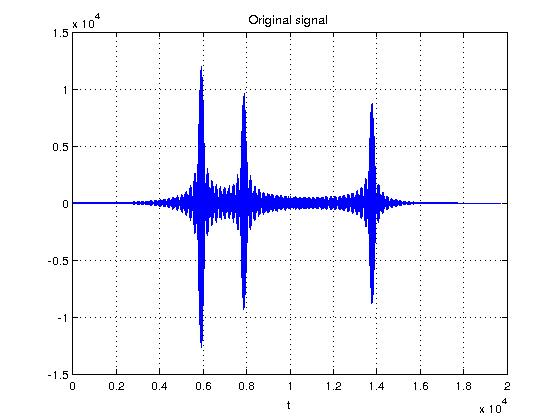
\includegraphics[height = 7.3 cm]{orig.jpg}
\caption{Original signal}
\label{orig_sigs}
\end{figure}

\begin{figure}[h]
\centering
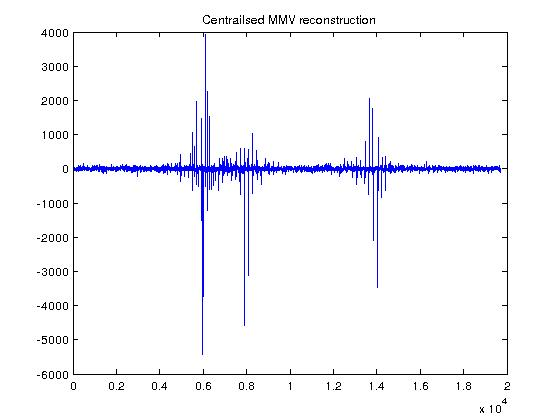
\includegraphics[height = 7.3 cm]{central_mmv.jpg}
\caption{ }
\label{central}
\end{figure}

\begin{figure}[h]
\centering
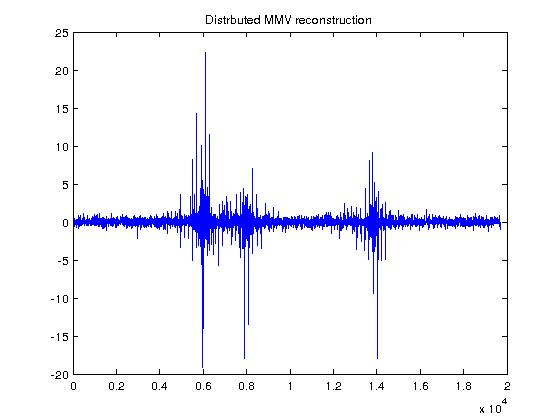
\includegraphics[height = 7.3 cm]{disrtrib_mmv.jpg}
\caption{ }
\label{distributed}
\end{figure}

\end{document}